\begin{icpcproblem}{B}{Battle for Silver}{Boaz Pat-El}{10}

Piet Hein was a Dutch naval officer during the Eighty Years' War between the United Provinces of The Netherlands and Spain.
His most famous victory was the capture of the \emph{Zilvervloot} (`Silver Fleet') near Cuba in 1628, where he intercepted
a number of Spanish vessels that were carrying silver from the Spanish colonies in the Americas to Spain.
Details about this famous naval battle are sketchy, so the description below may contain some historical inaccuracies.

The Silver Fleet consisted of vessels containing silver coins. Piet Hein's basic strategy was simple:
  tow away a number of vessels from the fleet, in order to capture their contents.

In an attempt to prevent the Dutch from carrying out this plan, the Spanish tied all the ships in their fleet together
using huge iron chains. Each vessel in their fleet was fixed to at least one other vessel; any two vessels
were connected by at most one chain; and the Spanish made sure that the chains did not cross each other, otherwise they
could get tied up into a knot. As an end result, the vessels and the chains connecting them formed a connected, planar graph.

However, the Spanish preventive measures only made their situation worse. As an experienced naval officer, Piet Hein knew that
towing away a group of ships was easiest if, for every two ships in the group, the ships were connected by a chain. He called
such groups \emph{chaingroups}.

Piet Hein ordered his men to tow away all the ships in the chaingroup that contained the largest amount of booty,
after severing the links with the remaining ships in the Spanish fleet with a few highly accurate canon shots.
The total booty in a chaingroup is the total number of silver coins in the vessels that make up the chaingroup.

%Figure \ref{fig:PietHein} visualizes this tactic.

\begin{figure}[h]
\centering
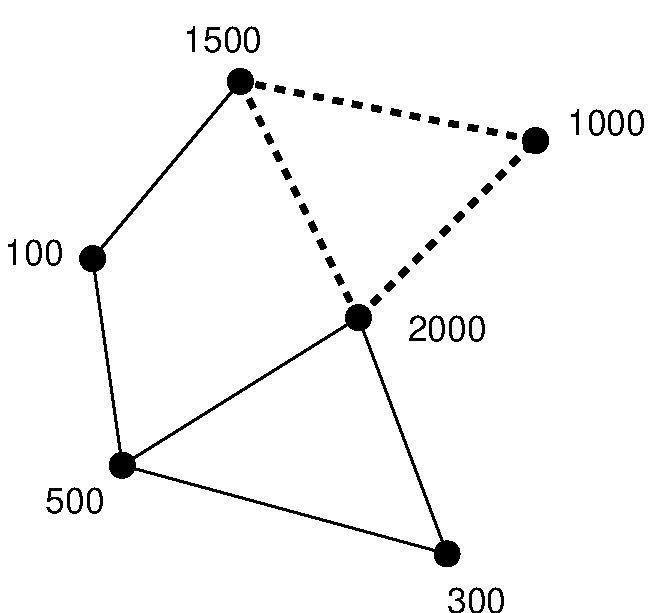
\includegraphics[width=0.38\textwidth]{piethein-diagram-dashed.pdf}
%\vspace{1mm}
\caption{The Silver Fleet represented as a graph: each dot denotes a vessel in the fleet, while each line denotes a chain that connects two vessels.
         The vessels that are connected in the figure by the dashed lines correspond to the chaingroup that provides the highest total value of silver coins.
         In this case, Piet Hein loots 4500 silver coins from the fleet.}
\end{figure}

\sectiontitle{Task}

Given a description of the Silver Fleet, find the value of the chaingroup with the highest amount of booty
(i.e., total number of silver coins in the ships that make up the chaingroup).

\sectiontitle{Input}

For each test-case:
\begin{itemize}
\setlength{\itemsep}{-1mm}
\item A line containing two integers $v$ $(2 \leq v \leq 450)$ and $e$ $(1 \leq e \leq 900)$, the number of vessels in the fleet and the number of chains, respectively.
\item Then, $v$ lines specifying $S_1, S_2, \ldots, S_v$, the amount of silver coins carried by vessel $i$ $(1 \le i \le v)$.
      The $S_i$ will be positive integers, where $100 \leq S_i \leq 6000$.
\item Then, for each chain, a line containing two integers $c_{start}$ and $c_{end}$,
      the two vessels connected by the chain, where ($1 \le c_{start} < c_{end} \leq v$).
\end{itemize}

Each fleet forms a connected, planar graph.

\sectiontitle{Output}

For each test case, one line containing a single positive integer: the number of silver coins that is captured by Piet Hein's fleet.

\sampleio{sample}

\end{icpcproblem}
